% PLEASE USE THIS FILE AS A TEMPLATE
% Check file iosart2c.tex for more examples
%
% Journal:
%   Journal of Ambient Intelligence and Smart Environments (jaise)
%   Web Intelligence and Agent Systems: An International Journal (wias)
%   Semantic Web: Interoperability, Usability, Applicability (SW)
% IOS Press
% Latex 2e

% options: jaise|wias|sw
% add. options: [seceqn,secfloat,secthm,crcready,onecolumn]


%\documentclass{iosart2c}

\documentclass[sw]{iosart2c}
%\documentclass[wias]{iosart2c}
%\documentclass[jaise]{iosart2c}

\usepackage[T1]{fontenc}
\usepackage[utf8]{inputenc}

\usepackage{times}%
\usepackage{natbib}% for bibliography sorting/compressing
%\usepackage{amsmath}
%\usepackage{endnotes}
%\usepackage{graphics}

%%%%%%%%%%% Put your definitions here
\usepackage{url}
\usepackage{graphicx}

\usepackage{ccicons}
\usepackage{relsize}
\newcommand{\uri}[1]{\textsf{\textscale{0.9}{#1}}}
%\newcommand{\uri}[1]{\textsf{\small{#1}}}
%%%%%%%%%%% End of definitions

\pubyear{2014}
\volume{0}
\firstpage{1}
\lastpage{1}

\newcommand{\ffbox}[1]{%
  {% open a group for a local setting
   \setlength{\fboxsep}{-2\fboxrule}% the rule will be inside the box boundary
   \fbox{\hspace{1.2pt}\strut#1\hspace{1.2pt}}% print the box, with some padding at the left and right
  }% close the group
}

\begin{document}

\begin{frontmatter}

%\pretitle{}
\title{DBnary: Wiktionary as a Lemon-Based Multilingual Lexical Resource in RDF}
\runningtitle{DBnary}
%\subtitle{}

\review{Sebastian Hellmann (AKSW, University of Leipzig); Steven Moran (LMU Munich); Martin Brümmer (AKSW, University of Leipzig); John McCrae (CITEC, University of Bielefeld)}{Hellmann Sebastian, Universität Leipzig, Germany; Eckle-Kohler Judith, Technische Universität Darmstadt, Germany; Gracia Jorge, Universidad Politécnica de Madrid, Spain}{}

% For one author:
\author{\fnms{Gilles} \snm{Sérasset}\thanks{E-mail: Gilles.Serasset@imag.fr.}}
\address{GETALP-LIG, UJF-Grenoble 1 \\BP 53, 38051 Grenoble cedex 9, France\\ \texttt{gilles.serasset@imag.fr}}
\runningauthor{Gilles Sérasset}

% Two or more authors:
%\author[A]{\fnms{} \snm{}\thanks{}},
%\author[B]{\fnms{} \snm{}}
%\runningauthor{}
%\address[A]{}
%\address[B]{}

\begin{abstract}
Contributive resources, such as Wikipedia, have proved to be valuable to Natural Language Processing or multilingual Information Retrieval applications. This work focusses on Wiktionary, the dictionary part of the resources sponsored by the Wikimedia foundation. In this article, we present our extraction of multilingual lexical data from Wiktionary data and to provide it to the community as a Multilingual Lexical Linked Open Data (MLLOD). This lexical resource is structured using the LEMON Model.\\
This data, called \textit{DBnary}, is registered at \url{http://thedatahub.org/dataset/dbnary}.
\end{abstract}

\begin{keyword}
Wiktionary \sep Multilingual \sep Lexical Resource \sep LEMON \sep Multilingual Linguistic LOD
\end{keyword}

\end{frontmatter}

\section{Introduction}

The GETALP (study group for speech and language translation/processing) team of the LIG (Laboratoire d'Informatique de Grenoble) is in need of multilingual lexical resources that should include language correspondences (translations) and word sense definitions. In this regard, the data included in the different Wiktionary\footnote{\url{http://www.wiktionary.org}} language editions is a precious mine.

Alas, many inconsistencies, errors and differences in usage do exist in the different Wiktionary language editions. Hence, we decided to make an effort to extract precious data from this source and provide it to the community as Linked Data. After a first version that used an RDF version of the LMF model \cite{FRANCOPOULO:2006:INRIA-00121468:1,francopoulo-EtAl:2006:MLRI} and was described in \cite{serasset:lrec2012}, we decided to adapt our extractors to the LEMON model \cite{McRae-lemon:2012}. This linked dataset won the ``Monnet-Challenge'' in 2012.

\section{Extracting data from Wiktionary}

\subsection{Motivation}

Errors and inconsistencies are inherent to a contributive resource like Wiktionary. Some language editions (like French and English) have many moderators who limit the number of inconsistencies among entries of the same language. These languages, which contain the most data, use many \textit{templates} that simplify the extraction process. For instance, the translation section of the French Wiktionary always uses a template to identify each individual translation (e.g. \ffbox{\texttt{\small \{\{trad+|de|Katze\}\} ''f''}} is the wiki code used for one of the German translations of the French word \emph{chat}).

This is not true anymore with less developed Wiktionary language editions. For instance, in the Finnish edition, some translations into French are introduced by the appropriate template (i.e. \ffbox{\texttt{\small\{\{fr\}\}}}) while others are introduced by the string \ffbox{\texttt{\small ranska}} which is the Finnish translation for "French". In this case, the extractor needs to know the Finnish translations of all language names to cope with the second case and avoid losing almost half of the available translation data.

Such inconsistencies and some errors in the data make the development of an extractor quite tedious. As many people in NLP are trying to use these data for different applications, we decided to extract lexical data from as many Wiktionary language editions as we could and provide it to the community while ensuring interoperability with other lexical data.

The DBnary extractor is written in java and is open-source (LGPL licensed, available at \url{http://dbnary.forge.imag.fr}). Anyone may contribute to this extraction effort by taking contact with the author.

\subsection{Scope of the extracted data}

The main goal of our efforts is not to extensively reflect the content of Wiktionary, but to create a lexical resource that is structured as a set of monolingual dictionaries complemented by bilingual translation information. This way, the structure of extracted data follows the usual structure of Machine Readable Dictionaries (MRD). We originally extracted those data as we needed translations in many languages along with textual definitions of senses that we used to compute semantic similarity between senses (using an adapted Lesk measure) for the Blexisma multilingual lexical disambiguation system \cite{schwab2012coling}.\footnote{We also used this dataset to build an UIMA component for word sense disambiguation, more details are available at \url{http://getalp.imag.fr/WSD}} Such data are already useful for several applications, but are merely a starting point for a future multilingual lexical database.

The monolingual data are always extracted from their own Wiktionary language edition. For instance, the French lexical data are extracted from the French language edition.\footnote{We use the term ``French language edition'' to refer to the data available on \url{http://fr.wiktionary.org}} Hence, we completely disregard the French data that may be found in other language editions.

We also filtered out some parts of speech in order to produce a result which is closer to existing monolingual dictionaries. For instance, in French, we disregard abstract entries that are prefixes, suffixes or flexions (e.g.: we do not extract data concerning \textit{in-} or \textit{-al} that are prefixes or suffixes and have a dedicated page in the French language edition).

\subsection{Availability of the extracted data}

DBnary data are made available using a Creative Commons Attribution-ShareAlike 3.0 license (\ccbysa). It may be downloaded from the DBnary website\footnote{\url{http://kaiko.getalp.org/about-dbnary}} as a set of turtle files (one per language).

As the Wiktionary language editions constantly evolve with entry modifications and additions, the DBnary dataset also evolves. Each time the Wikimedia foundation provides a new dump\footnote{dumps are available at \url{http://dumps.wikimedia.org/}.} of a Wiktionary language edition, DBnary data are extracted with the new dump and made available online. Older versions are kept and remain available for further reference. At the time of writing, the dumps are updated about once every ten days for each language. 

DBnary data are also available as Linguistic Linked Open Data (LLOD). All DBnary IRIs are dereferencable and a SPARQL endpoint is available at \url{http://kaiko.getalp.org/sparql}. However, as the DBnary data change almost everyday, the data that is available this way is not necessarily up to date.

\subsection{Interlinking}

Our work focuses only on the lexical data. Hence, we do not provide any reference to any ontology. Moreover, in this dataset, we only try to \emph{extract} lexical data from Wiktionary, but we do not try(yet) to \emph{enrich} it. Hence, this dataset is not (at the time of printing) linked to other lexical linked data. 

Also, any interlinking with DBnary data will require that we take into account the constantly evolving nature of the dataset that changes every two days on average (as Wikimedia dumps are made available). Indeed, there is a chance that URIs of lexical senses may change between two versions as word senses may be reordered in the original Wiktionary data.\footnote{Strictly speaking, even URIs of lexical entries may change, but this is even more unfrequent.} We believe that such changes are rather unfrequent, but we still have to find out a way to cope with them. 

As the DBnary data have been extracted regularly since almost one year, with about 25 different versions per language, diachronic studies may now be performed to evaluate the frequency of such changes. However, such studies are not trivial to implement as a change in a definition does not necessarily imply that the lexical sense has changed.

\section{Extracted Data as a LEMON Lexical Resource}

\begin{figure*}[tbp]
\resizebox{\linewidth}{!}{%
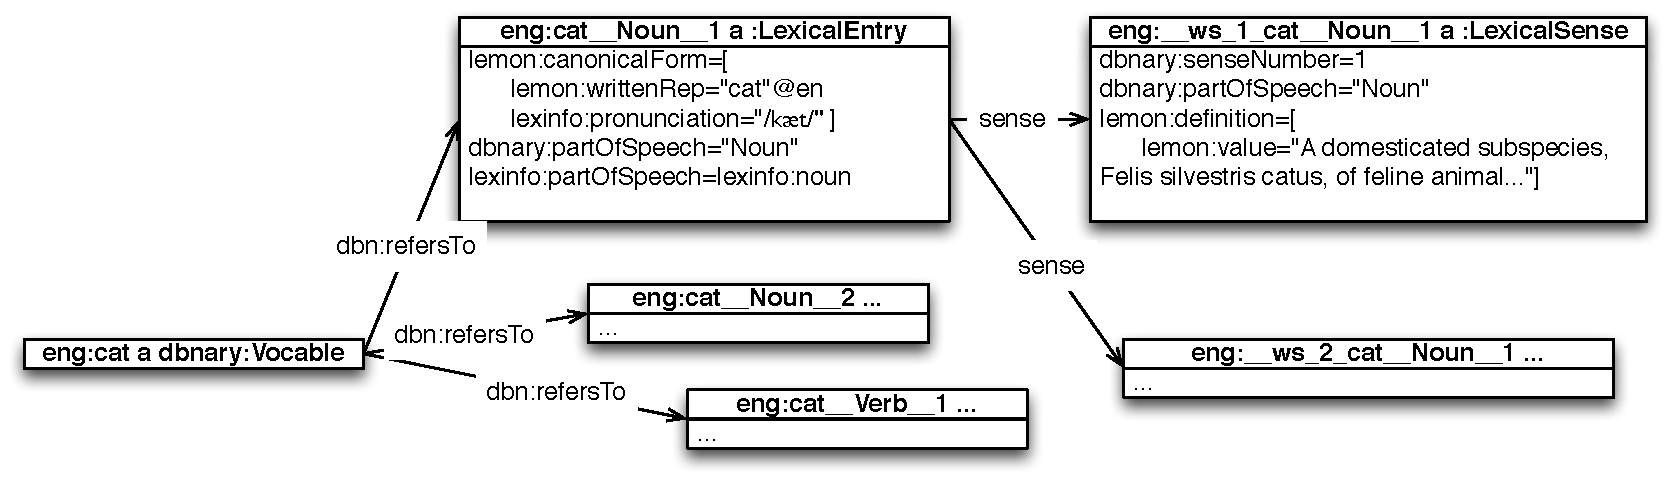
\includegraphics{cat_struct.pdf}
}
\caption{An extract of the DBnary entry "cat" in English, showing the respective roles of \uri{Vocable}, \uri{LexicalEntry} and \uri{LexicalSense} in the DBnary dataset.}\label{dbnary:cat}
\end{figure*}

\begin{figure*}[tbp]
\resizebox{\linewidth}{!}{%
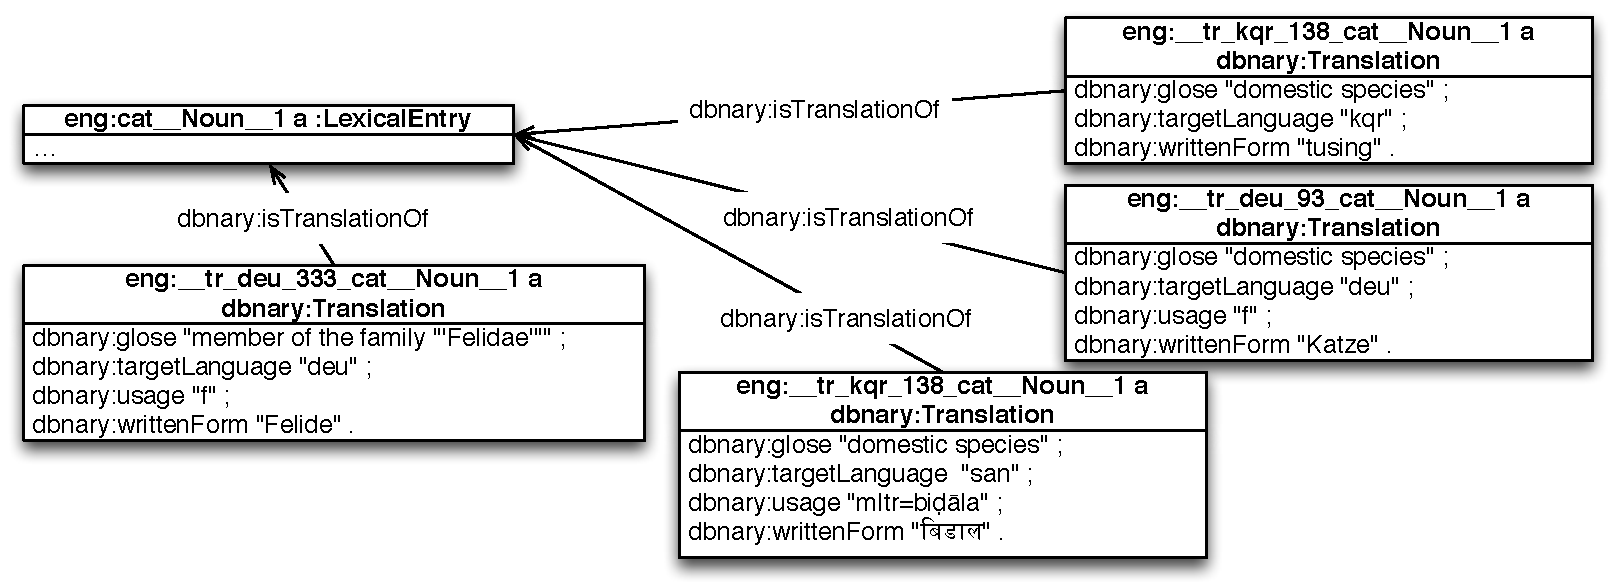
\includegraphics{cat_translations.pdf}
}
\caption{A subset of the translations related to the lexical entry \uri{eng:cat\_Noun\_1}.}\label{dbnary:catequiv}
\end{figure*}

\subsection{Using LEMON for legacy lexical data}

The LEMON model itself is not sufficient to represent lexical data that are currently available in classical monolingual and bilingual dictionaries. For instance, LEMON does not contain anything to represent translations between languages as it assumes that such a translation will be handled by the ontology description. Moreover, LEMON assumes that all data is well-formed and fully specified. As an example, the synonymy relation is a property linking a \uri{LexicalSense} to another \uri{LexicalSense}. While it is correct to assume as a \textit{principle}, this does not account for the huge amount of legacy data that is available in dictionaries and lexical databases.

As an example, in the English language edition, one may find a synonymy relation between \textit{cat\_n} and \textit{bitch}. This relation links a \textit{Lexical Entry} with a \textit{Vocable}. Creating a corresponding lexico-semantic relation from \textit{Lexical Sense} to \textit{Lexical Sense} would imply: (1) detecting the correct sense of \textit{cat\_n} (here sense \#4/15); (2) deciding which is the target lexical entry (here, \textit{bitch} has 2 lexical entries, but only one is nominal); (3) deciding which lexical sense it is (\#2/9). As such a process is error prone, we decided to provide the data as they appear in Wiktionary and to leave these decisions to further processing.

In order to cope with these legacy data, we extended the LEMON model by adding new classes and properties. However, when a piece of data is representable as a LEMON entity, then we do it. Moreover, when possible, we use the ISOcat registry \cite{DBLP:books/daglib/p/WindhouwerW12} to identify standard elements in the lexical data.

\subsection{DBnary extension to LEMON}

The LEMON model has been extended to cope with legacy lexical data. Added classes and properties are:

\begin{description}
\item[Vocable:] Several lexical entries may be contained in a single Wiktionary page, and most lexical relations are simply targeted to Wiktionary pages. Hence, we introduced the \uri{dbnary:Vocable}\footnote{The \uri{dbnary} namespace used in this article resolves to \url{http://kaiko.getalp.org/dbnary#}} class to represent a Wiktionary page, as a reification of the set of Lexical entries it contains. This class is a subclass of \uri{lemon:LexicalEntry}. Instances of that class are related to their lexical entries through the \uri{dbnary:refersTo} property. 

\item[LexicalEntity:] Lexical relations should usually link two \textit{Lexical Senses}. However, most relations found in legacy lexical data are underspecified. Some relations link a \textit{Lexical Sense} to a \textit{Vocable} or to a \textit{Lexical Entry}. Others even link two \textit{Lexical Entries}. In order to cope with such underspecified relations, we introduced the \uri{dbnary:LexicalEntity} class which is the union of  \textit{Lexical Entry} and \textit{Lexical Sense}.\footnote{Indeed, we could have simply defined the domain/range of lexical relations and translations as a \uri{owl:unionOf} \textit{Lexical Entry} and \textit{Lexical Sense}.}

\item[Nyms:] Most Wiktionary language editions provide ``nymy'' relations (mainly synonymy, antonymy, hypernymy, hyponymy, meronymy and holonymy), that are almost always underspecified. Hence, DBnary introduces 6 new ``nymy'' properties (in \uri{dbnary} name space). The  domain and range of these relations are \textit{Lexical Entities}.

\item[Translations:] As there is no way to represent bilingual translation relations in LEMON, we introduced the \uri{dbnary:Translation} class that collects translation information contained in Wiktionary. This class admits several properties:
\begin{itemize}
\item \uri{dbnary:isTranslationOf} relates the translation to its source \textit{lexical Entity} (i.e. either a Lexical Sense, or a Lexical Entry). 
\item \uri{dbnary:targetLanguage} is an object property whose range is a \texttt{dcterms:\-Linguistic\-System}. All values are in the \emph{lexvo} name\-space.\footnote{e.g. \uri{http://lexvo.org/id/iso639-3/deu} represents the German language}
\item \uri{dbnary:writtenForm} gives the written form of the translation in the target language. We decided not to relate it to a vocable as some translations may not be definable as lexical entries in the target language.
\item \uri{dbnary:gloss} is a string property that contains all available information used to denote the lexical sense of the source of the translation (e.g. in the English entry "cat", the German translation "Katze" appears in a box labelled with the \textit{gloss} "domestic species", used to denote the fact that "Katze" is a translation of the \textit{Lexical Sense} defined by "A domesticated subspecies, Felis silvestris catus, of feline animal...".\footnote{This means that, in an ideal situation, the translation should be linked to this \textit{Lexical Sense}, instead of the \textit{Lexical Entry}, however, such a linking may be error prone, hence, we decided to make such refinements afterwards.}
\item \uri{dbnary:usage} is a string property that contains all available information concerning this translation object. It usually gives additional information on the target entry.
\end{itemize}

\end{description}

\subsection{Structure of the extracted lexical data}



Figure \ref{dbnary:cat} illustrates the main elements characterizing a lexicon entry in the DBnary data. Each Wiktionary page is represented by a \uri{dbnary:Vocable} element that refers to its corresponding \uri{lemon:Lexical\-Entry}. Each lexical entry corresponds to one lemma, one etymology and one part of speech. Each lexical entry is related to its \uri{lemon:Lexical\-Sense} by the \uri{lemon:sense} property. A lexical sense corresponds to one definition. 

Each lexical entry is related to its canonical form and possibly to alternate forms (that are represented using \uri{lemon:LexicalForm}s). The part of speech is available through the \uri{dbnary:partOfSpeech} property that gives the part of speech as defined by the Wiktionary language edition, and through the \uri{isocat:partOfSpeech} property that points to a standard ISOcat part of speech value.

\begin{figure*}[tbp]
\resizebox{\linewidth}{!}{%
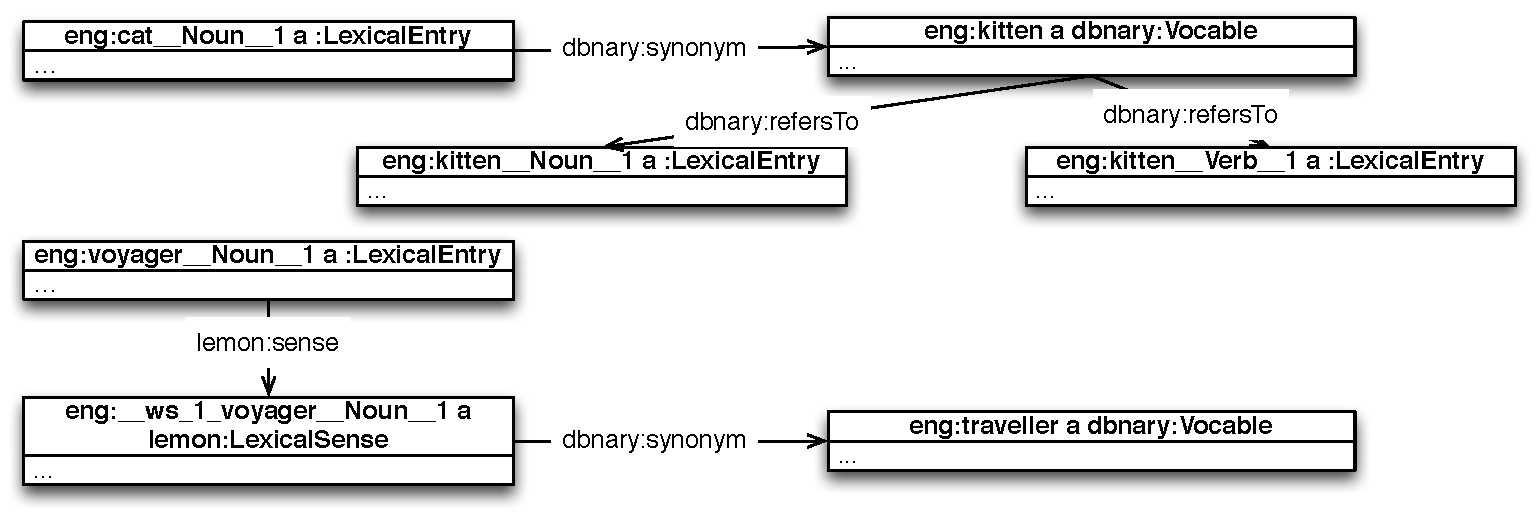
\includegraphics{cat_syn.pdf}
}
\caption{An example of a synonymy relation for the lexical entry \uri{eng:cat\_Noun\_1}.}\label{dbnary:catsyn}
\end{figure*}


Figure \ref{dbnary:catequiv} illustrates the \textit{DBnary} extension to LEMON that is used to represent the numerous translations available in Wiktionary. Each translation is represented as a \uri{dbnary:Translation} instance associated to a \textit{lexical entry} by the \uri{is\-Translation\-Of} property. The translation is given as a string through the \uri{writtenForm} property, as some translations may not necessarily correspond to vocables in the target language (e.g. explanatory translations). The target language of the translation is given using the ISO 639-3 3-letter language code \cite{ISO639-3:2007}. When available, the \uri{gloss} property value gives an indication concerning the lexical sense that is translated. In the current dataset, the translation is linked to a usually ambiguous lexical entry and the \textit{gloss} is kept for further attachment to the correct word sense.

Wiktionary contains many thesaurus relations (like synonymy, antonymy, etc.) that are represented using the above mentioned ``nymy'' properties which relate a \textit{lexical entity} with another \textit{lexical entity}. In the current dataset, most of the property subjects are \textit{lexical entries}. However, in the case of monosemous lexical entries, the synonymy relation is attached to the unique \uri{lemon:LexicalSense}. Figure \ref{dbnary:catsyn} illustrates how DBnary encodes ``nymy'' relations with examples of the \uri{dbnary:synonym} property. The upper part of the figure shows an example of a \uri{dbnary:synonym} property that is related to the ambiguous lexical entry \uri{eng:cat\_\_Noun\_\_1}. The lower part shows that, in the monosemous lexical entry \uri{eng:voyager\_\_Noun\_\_1}, the \uri{dbnary:synonym} property is related to the unique lexical sense of the entry. The object of such properties are always \uri{dbnary:Vocable}.


\section{Size and quality of the involved data}

All sizes indicated in this section reflect the state of the DBnary data at the time of writing (June 2013). These numbers are constantly evolving, as the original Wiktionary data is edited and as the extractor itself is improved.\footnote{Statistics concerning the latest extracts will be made available on the DBnary website.}
 Table \ref{globalsize} gives the size of the resources available in DBnary for the 8 languages currently extracted.\footnote{The currently extracted languages are (by increasing order of the ISO 639-3 language codes):
German (deu),
Greek (ell),
English (eng),
Finnish (fin),
French (fra),
Portuguese (por),
Russian (rus),
}

\begin{table}[htb]
\begin{tabular}{lrrrr}
 & \textbf{Entries} & \textbf{Vocables} & \textbf{Senses} & \textbf{Translations}\\
 \hline
\textbf{eng} & 527067 & 504594 & 421232 & 1126463 \\
\textbf{fra} & 273822 & 283847 & 358921 & 464956 \\
\textbf{deu} & 135103 & 201736 & 95593 & 471892 \\
\textbf{rus} & 127271 & 139235 & 99243 & 325345 \\
\textbf{ell} & 74056 & 74800 & 34932 & 55652 \\
\textbf{fin} & 48164 & 48050 & 56559 & 118728 \\
\textbf{por} & 43042 & 44061 & 77631 & 225065 \\
\textbf{ita} & 25279 & 31935 & 35061 & 57796 \\
\end{tabular}
\caption{Number of resources by type and language, sorted by number of lexical entries.}\label{globalsize}
\end{table}



Table \ref{nymsize} gives an overview of the number of lexico-semantic relations available in each language edition.

\begin{table}[htb]
\begin{tabular}{lrrrrrr}
 & \textbf{syn}  & \textbf{ant} & \textbf{hyper} & \textbf{hypo} & \textbf{mero} & \textbf{holo} \\
 \hline
\textbf{eng} & 31461& 6877& 959& 1103& 114& 0 \\ 
\textbf{fra} & 30088& 6735& 8215& 3557& 943& 1847 \\ 
\textbf{deu} & 27516& 14315& 30202& 9509& 0& 0 \\ 
\textbf{rus} & 22631& 9204& 21028& 4756& 0& 0 \\ 
\textbf{ell} & 3975& 1116& 0& 0& 0& 0 \\ 
\textbf{fin} & 2255& 0& 0& 0& 0& 0 \\ 
\textbf{por} & 3527& 575& 6& 3& 0& 0 \\ 
\textbf{ita} & 7091& 2337& 0& 0& 0& 0 \\ 
\end{tabular}
\caption{Number of lexico-semantic relations. Languages are sorted according to their number of lexical entries.}\label{nymsize}
\end{table}

\begin{table}[htb]
\begin{tabular}{lrr}
\textbf{language} & \textbf{\# of transl.}\\
 \hline
\textbf{eng} & 5110 (.991) \\
\textbf{fra} & 5799 (1.070) \\
\textbf{deu} & 10287 (.992)\\
\textbf{rus} & 8436 (248.117) \\
\textbf{ell} & 2598 (.643) \\
\textbf{fin} & 7245 (289.80) \\
\textbf{por} & 17720 (.932) \\
\textbf{ita} & 7855 (31.673) 
\end{tabular}
\caption{Extracted translations vs interwiki links ratio, on a random sample of 1000 entries.}\label{iwlinks}
\end{table}

Table \ref{tradsize} shows the number of translations available in each language edition, for the 8 currently extracted languages. It also gives the total number of translations and the number of the different target languages with translations. Not surprisingly, the English language edition shows the largest number of translations to more than 1000 different languages. 

\begin{table*}[htb]
\begin{tabular}{lrrrrrrrrrrrrr}
\textbf{Source/Target}  & \textbf{deu} & \textbf{ell} & \textbf{eng} & \textbf{fin} & \textbf{fra} & \textbf{ita} & \textbf{por} & \textbf{rus}& \textbf{others} & \textbf{Total} & \textbf{\# of target languages}\\
\textbf{eng} & 62501 & 23794 & 1 & 74938 & 57959 & 37467 & 30256 & 74837 & 764710 & 1126463 & 1143\\
\textbf{fra} & 34608 & 7063 & 74687 & 7589 & 12 & 18806 & 17784 & 7783 & 296624 & 464956 & 952\\
\textbf{deu} & 0 & 2675 & 81015 & 4947 & 67143 & 41485 & 8872 & 17354 & 248401 & 471892 & 355\\
\textbf{rus} & 23056 & 3295 & 48559 & 3966 & 14776 & 12643 & 5567 & 0 & 206709 & 318571 & 490\\
\textbf{ell} & 2242 & 2 & 10090 & 1056 & 8436 & 1470 & 1149 & 1315 & 29892 & 55652 & 246\\
\textbf{fin} & 8046 & 918 & 30103 & 0 & 6700 & 3856 & 2196 & 7997 & 58912 & 118728 & 329\\
\textbf{por} & 7000 & 2816 & 11284 & 4607 & 8720 & 7096 & 4 & 4396 & 179142 & 225065 & 695\\
\textbf{ita} & 4619 & 506 & 17539 & 925 & 4461 & 75 & 1219 & 938 & 27514 & 57796 & 315\\
\end{tabular}
\caption{Number of translations from/to the 8 currently extracted languages. Source languages are sorted according to their number of lexical entries. Target languages are sorted by their ISO 639-3 language code. The number of different target languages is also given.}\label{tradsize}
\end{table*}

Asserting the quality of the extracts is difficult. We may compare the data with other Wiktionary extraction initiatives like \cite{Zesch08Wikipedia} (contained in UBY \cite{UBY:TUD-CS-2012-0023}) or Wiktionary2RDF \cite{DBLP:conf/aswc/HellmannBA12}. But this will only give informations regarding the common extracted languages. 

In order to guide the extractors definition and maintenance, we compare the extracted data with the count of interwiki links\footnote{Interwiki links are links going from one Wiktionary language edition to another. This count is a rough estimate of the translations available in an entry.} (available through a Wiktionary API). Table \ref{iwlinks} gives an overview of such a comparison. Column \textit{\# of transl.} shows the number of extracted translations and the ratio of extracted translations vs interwiki links. As may be seen, the Greek extractor only gets a 0.64 ratio of extracted translations vs interwiki links. This is an indication of the fact that this extractor is in a very rough state. On the contrary, the French extractor gets more translations than interwiki links, as the French edition does not generate links when the target language edition does not exist. Such heuristics are not applicable to the Finnish and Russian editions as they do not use interwiki links for their translations.

Finally, by comparing the evolution of extracted data over time, we are able to detect when an editorial decision is made in a language edition that leads to a loss of extracted data. That was the case when the French language editors decided to change the names of the macros used to represent a translation. 

\section{Conclusion and Perspectives}

We have presented the DBnary dataset, a LEMON-based lexical network built from different Wiktionary language editions. That work is interesting for many users as it enables them to use the extracted data in their own NLP systems. Moreover, as the extracted resource uses the Resource Description Framework (RDF) standard and the LEMON model, the extracted data are also directly usable by researchers working on the Semantic Web, where it could be used to ease the ontology alignment systems when terms in different languages are used to describe ontologies of a domain.

DBnary contains a significant number of entries for at least English and French, which makes it comparable to Wordnet \cite{wordnet-fellbaum}. Moreover, it contains many translations with certain language pairs that makes it also comparable to the Open Multilingual Wordnet \cite{DBLP:conf/acl/BondF13} (an aggregation of several existing multilingual Wordnets).

Our next objective is to better generalize the treatments of the current extractors, so that it will be easier to create and maintain extractors for other languages. We have recently introduced extractors for the Russian and Greek languages, and are working on others. We welcome all initiatives aiming at the addition of new languages to this open-source tool. 

We will also enhance the \textit{DBnary} data by providing more lexico-semantic relations and translations linked on the lexical sense level.

\section{Acknowledgements}

The work presented in this paper was conducted in the Videosense project, funded by the French National Research Agency (ANR) under its CONTINT 2009 programme (grant ANR-09-CORD-026).

%%%%%%%%%%% The bibliography starts:
\bibliographystyle{abbrvnat}      % basic style, author-year citations
\bibliography{biblio}   
%\begin{thebibliography}{9}

%\bibitem{r1}

%\bibitem{r2}

%\end{thebibliography}

\end{document}
